\documentclass{IEEEtran}
\usepackage{graphicx}
\usepackage{caption}
\usepackage{lipsum}
\usepackage{listings}
		
\author{Alp Gokcek, Erdal Sidal Dogan, Mert Komurcuoglu\\\{gokcekal, doganer, komurcuoglum\}@mef.edu.tr\\ MEF University \\ \today}
\title{Rock-Paper-Scissors AI Agent}


\begin{document}
	\maketitle
	\section{Introduction}
	
	Rock-Paper-Scissors is a game that has been around for while and well known to almost everyone. The game is played with two players, goal is to defeat the opponent by making a choice that prevails the opponents. Rules to defeat is as follows;
	
	\begin{enumerate}
		\item Paper\textgreater Rock
		\item Rock\textgreater Scissors	
		\item Scissors\textgreater Paper
	\end{enumerate}
	
	In the beginning of the game, two players make a random choice among the Rock-Paper-Scissor triplet simultaneously. Whoever made the choice that defeats the opponents choice wins the game.
	
	Even though it seems that the choices are random and probabilities of winning for each player is equal, scientist discover that "if a player wins for a round, they are much more likely to win to following one too".Furthermore, the choices that players make are prone to biases. \cite{winning-rps} 
	
	\section{Solution Design Process}
	
	For this problem, our initial approach was to design a rule based system where the each case was covered with the if-else statements. Later on, we searched for another applicable method that we have covered in the lecture so far. Upon our researches, we decided to use \textit{Discrete Markov Chains}
	
	\textit{DMC} methods suggest creating a \textit{State Transition Matrix}. Each column of the matrix is the probability score of the upcoming move of the opponent; rows of the matrix corresponds to a previous set of plays and stochastic. \\
	
	UML Diagram of the \texttt{RPS\_Agent} class can be seen from Figure \ref{UML}.
	
	\begin{table}[h!]
		\begin{center}
					\caption{Transition Matrix with initial transition values}
			\begin{tabular}{c | c  c  c}
				State &  R & P & S \\
				\hline
				RRR & 0.333 & 0.333 & 0.333 \\
				RRP & 0.333 & 0.333 & 0.333 \\
				RRS & 0.333 & 0.333 & 0.333 \\
				\vdots \\
				SSS & 0.333 & 0.333 & 0.333 \\
			\end{tabular}
		\end{center}
	\end{table}
	
	\section{Implementation}
	
	The program has been implemented with \textit{Python Language}. In order to have concise structure in the program, we defined our AI Agent as an object. This class, consist of transition matrix and all the complementary methods such as create matrix, update matrix etc.
	
	Most important function and variables in this class are as follows; \texttt{update\_transition\_matrix(), predict()}
	
	\subsection{Update Transition Matrix}
		The program makes probability calculations relying on last 3 moves of the opponent, hence, before this calculations game must be played at least three times. This method checks the game has played for at least 3 rounds, if not, doesn't update the matrix at all. Otherwise, it multiplies each value on the row with a predefined \texttt{decay} value in order to reduce the weight of the earlier moves and increase the effect of the last move on the probability score.
		
		Finally, it updates the \texttt{transition\_sum\_matrix} where the number of occurrence for the each case is stored. As the \texttt{transition\_sum\_matrix} is updated, new probability scores are calculated on the \texttt{transiton\_matrix}
		

		
		
		\lstinputlisting[language={Python}, frame=single, breaklines, basicstyle=\ttfamily, caption= \texttt{update\_transition\_matrix()} method]{source-codes/update-transition-matrix.py} \label{update-matrix-code}

	\subsection{Predict}
		This method predicts the opponents move.
	
		Since we don't have any data to make our predictions to be based on, in the initial predictions we used the statistics that psychologists observed when conduction a research about the human behavior on Rock-Paper-Scissors.  
		
		For the later moves, we use the transition matrix as lookup table where the row corresponding the last 3 moves presents us with the probabilities of the next move. Intuitively, we choose the next state with the highest probability score. However, if one of the scores are significantly higher than the others, we assume that it will be predicted by our opponent agent and it will make their move accordingly. In order to protect ourselves from this move, we make the move with least probability score to surprise the opponent. 
				
		\lstinputlisting[language={Python}, frame=single, breaklines, basicstyle=\ttfamily, caption=\texttt{predict()} method]{source-codes/predict.py} \label{predict-code}
	
	\begin{figure}
		\centering
		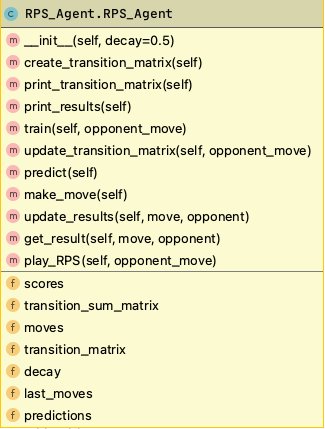
\includegraphics[scale=0.5]{RPS_Agent.png}
		\caption{"UML Diagram of the RPS Agent Class"}\label{UML}
	\end{figure}
	
	
	\section{Testing}
		During the testing stage, we saw that our initial approach where the outcome with the highest probability is chosen and if there is a significant gap with other options, our predictions would be obvious to the opponent as well. Thus, we've implemented a system that will take precautions by reverting the probability scores by subtraction from 1 and converting the least likely one to be the most likely. By this approach, we increased our chances against the intelligent systems.
		
		In this stage, we've also tested for different values of the \texttt{decay} value. Our observations indicated that the highest success value is reached when the decay has taken values between the $0.4-0.6$ range. We chose the set this value to $0.5$
		
		Below you can see the outcomes of the 10 games of 1000 rounds with two kinds of opponents;
		
			\begin{figure}[h!]
				\centering
				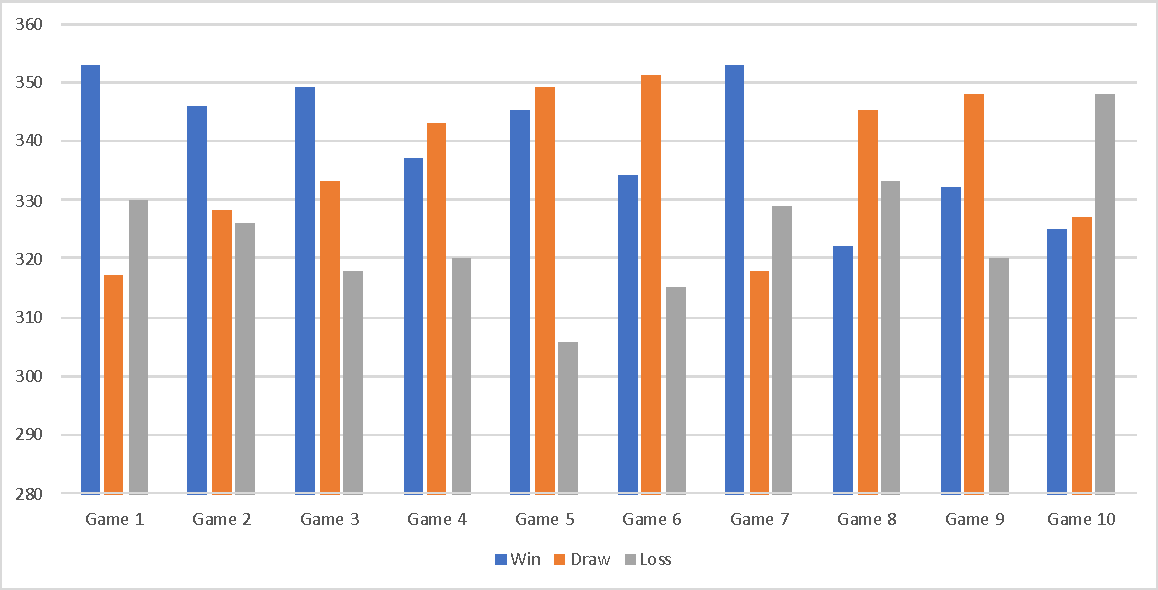
\includegraphics[scale=0.4]{fully-random.pdf}
				\caption{"Distribution of outcomes when playing against randomly deciding opponent"}\label{fand}
			\end{figure}


			\begin{figure}[h!]
				\centering
				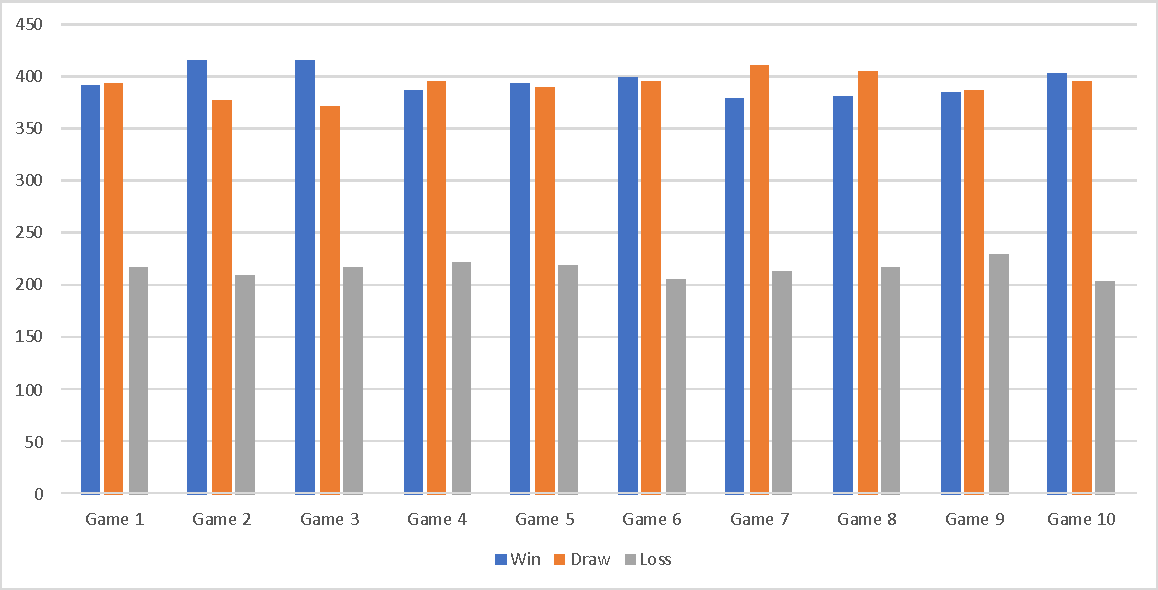
\includegraphics[scale=0.4]{rule-based.pdf}
				\caption{"Distribution of outcomes when playing against the intelligent opponent that uses rule-based approach"}\label{fand}
			\end{figure}


		\pagebreak

	\section{Teamwork}
	
	Most of the implementation is carried out by Alp \& Mert, Erdal has contributed on the testing stage and forming a report. 

	\bibliographystyle{IEEEtran}
	\bibliography{ref.bib}
	
\end{document}
